%-----------------------------------------------------------------------------%
\chapter{\babTiga}
%-----------------------------------------------------------------------------%
%\todo{tambahkan kata-kata pengantar bab 1 disini}


%-----------------------------------------------------------------------------%
\section{Metodelogi Peneltian}
%-----------------------------------------------------------------------------%

Pada penelitian kali ini dilakukan langkah-langkah secara terencana dan sistematis, hal ini berguna agar dapat mempermudah proses dalam pengerjaan penelitian. Metode yang digunakan dalam penelitian ini menggunakan metode tindakan karena dari tujuan peneltian ini agar memperoleh model \scm yang paling efektif dan efisien dalam mengelola bisnis dalam perusahaan atau organisasi. Adapun tahapan penelitian adalah terlihat \pic~\ref{fig:alurPenelitian} pada sebagai berikut :
\begin{figure}
	\centering
	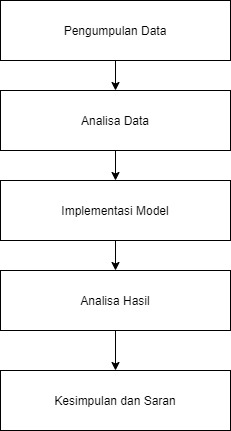
\includegraphics[width=0.40\textwidth]
		{pics/alur-penelitian.jpg}
	\caption{Metodelogi Penelitian}
	\label{fig:alurPenelitian}
\end{figure}


%-----------------------------------------------------------------------------%
\section{Pengumpulan Data}
%-----------------------------------------------------------------------------%
Pada Pada tahap pengumpulan data, penelitian ini menggunakan data primer pada sistem informasi penjualan Toko Chaca Komputer. Data yang digunakan pada penelitian ini adalah berupa data transaksi penjualan, data produk, data kategori produk dan data pelanggan. Data-data tersebut digunakan sebagai variabel-variabel yang signifikan maupun variabel pembantu yang saling berpengaruh untuk pemodelan sistem yang akan disimulasikan. Data yang terkumpul untuk selanjutnya dianalisis dan akan digunakan sebagai bahan dalam tahapan selanjutnya yaitu analisa data.

%-----------------------------------------------------------------------------%
\section{Analisa Data}
%-----------------------------------------------------------------------------%

Pada tahap analisa data, penelitian ini menggunakan data yang telah di kumpulkan untuk di analisa ulang yang akan disesuaikan dengan kebutuhan untuk kepada tahap selanjutnya.

%-----------------------------------------------------------------------------%
\section{Implementasi Model}
%-----------------------------------------------------------------------------%
Implementasi model merupakan implementasi dari data yang telah di analisa kemudian di implementasi ke model yang telah di kembangkan yang bertujuan untuk menguji model yang digunakan.

%-----------------------------------------------------------------------------%
\section{Analisa Hasil}
%-----------------------------------------------------------------------------%
Setelah melakukan implementasi model, maka tahapan yang selanjutnya dilakukan adalah melakukan analisa terhadap hasil simulasi dari pengembangan awal model sistem yang telah dibuat, kemudian dilakukan perbaikan terhadap model awal berdasarkan hasil skenario yang telah diuji coba.

%-----------------------------------------------------------------------------%
\section{Kesimpulan dan Saran}
%-----------------------------------------------------------------------------%

Tahap penyusunan kesimpulan dilakukan dengan menelaah secara keseluruhan terhadap apa yang telah dilakukan pada penelitian ini. Kesimpulan dibuat berdasarkan hasil studi literatur, desain metode penelitian, validasi data, analisis hasil simulasi dan penyusunan hasil yang diperoleh dari pengembangan model dan sistem rantai pasok barang berdasarkan produk pada toko chaca komputer. Tahap terakhir dalam penelitian ini juga menganalisis dan membahas temuan keseluruhan dalam penelitian, terkait dengan kesimpulan hasil pengujian model sistem dinamik dan saran untuk peluang penelitian yang akan datang. 